The primary transformed grid revealed nonnested LCC paths in 554/701 images (79.0\%) and adjacent increases in annotated-area loss in 497/701 (70.9\%; Table~\ref{tab:data}). The two quantities differ because deleted pixels need not intersect the reference annotation. Figure~\ref{fig:mechanism} isolates the mechanism in an exact synthetic example.

\begin{figure}[htbp]\centering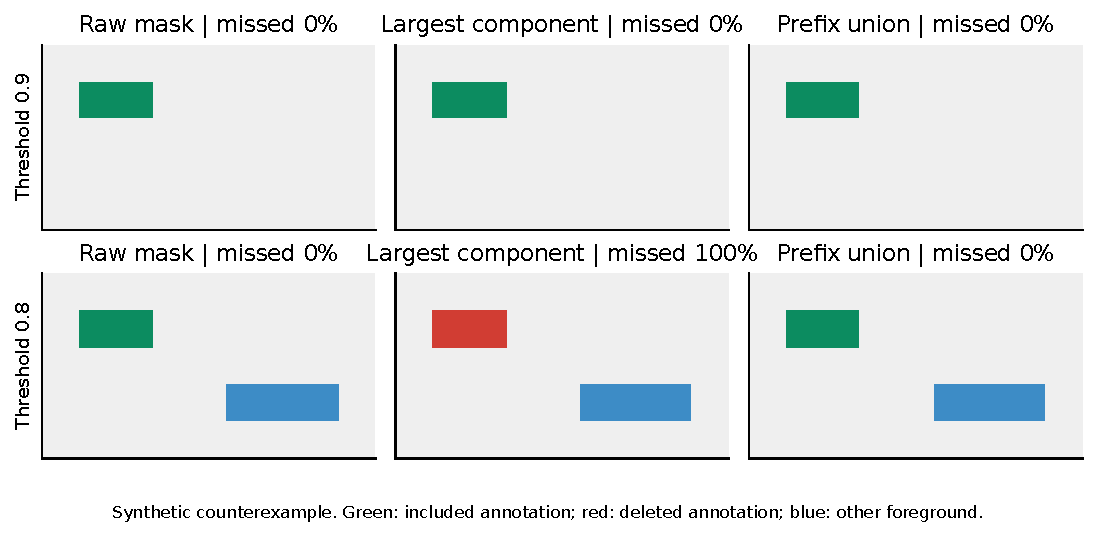
\includegraphics[width=.94\linewidth]{../figures/mechanism.pdf}\caption{A synthetic switch between two disconnected regions. Lowering the threshold adds pixels to the raw mask but replaces its largest component. The two-pixel reference annotation is then lost. The running union retains it. Colors distinguish annotated foreground from other selected pixels.}\label{fig:mechanism}\end{figure}

\subsection{Cleanup after raw calibration}
Across the shared splits, raw CRC attained mean missed area 9.36\%, whereas subsequent LCC cleanup increased it to 48.64\% (Table~\ref{tab:primary}). The paired increase was 39.29 percentage points. Cleanup removed more than 1\% of annotated area in a mean 45.42\% of evaluation images. The predicted frame area changed from 33.17\% to 23.89\%, a decrease in displayed area accompanied by a substantial recall cost. These are properties of the sampled images, not estimates of clinical polyp miss rate.

At the descriptive full-pool calibrated threshold $t=5.7e-05$, the mean per-image cleanup penalty was 41.82 percentage points (image-bootstrap 95\% interval 38.31--45.39). In 336 images the penalty exceeded one percentage point. This threshold uses the entire pool and is not a held-out operating-point estimate.

\begin{table}[htbp]\centering\small
\caption{PraNet primary evaluation at target 10\% missed annotated area. Values average 500 shared splits, with 350 calibration and 351 evaluation images. The range is the 2.5th--97.5th percentile of split risks, not a population confidence interval. All numerical columns except Dice are percentages.}
\label{tab:primary}
\begin{tabular}{lrrrr}\toprule
Procedure & Missed area & Split range & Frame area & Dice\\\midrule
Raw CRC & 9.36 & 6.39--13.51 & 33.17 & 0.345 \\
Raw CRC + LCC & 48.64 & 29.39--62.81 & 23.89 & 0.321 \\
LCC recalibration & 9.16 & 5.56--14.13 & 92.54 & 0.135 \\
Prefix union CRC & 8.99 & 5.42--12.69 & 39.43 & 0.300 \\
LCC envelope CRC & 9.16 & 5.56--14.13 & 92.54 & 0.135 \\
Anchor CRC & 9.01 & 5.10--12.47 & 28.01 & 0.579 \\
Area opening CRC & 9.35 & 6.41--13.57 & 33.35 & 0.343 \\
\bottomrule\end{tabular}\end{table}
\begin{figure}[htbp]\centering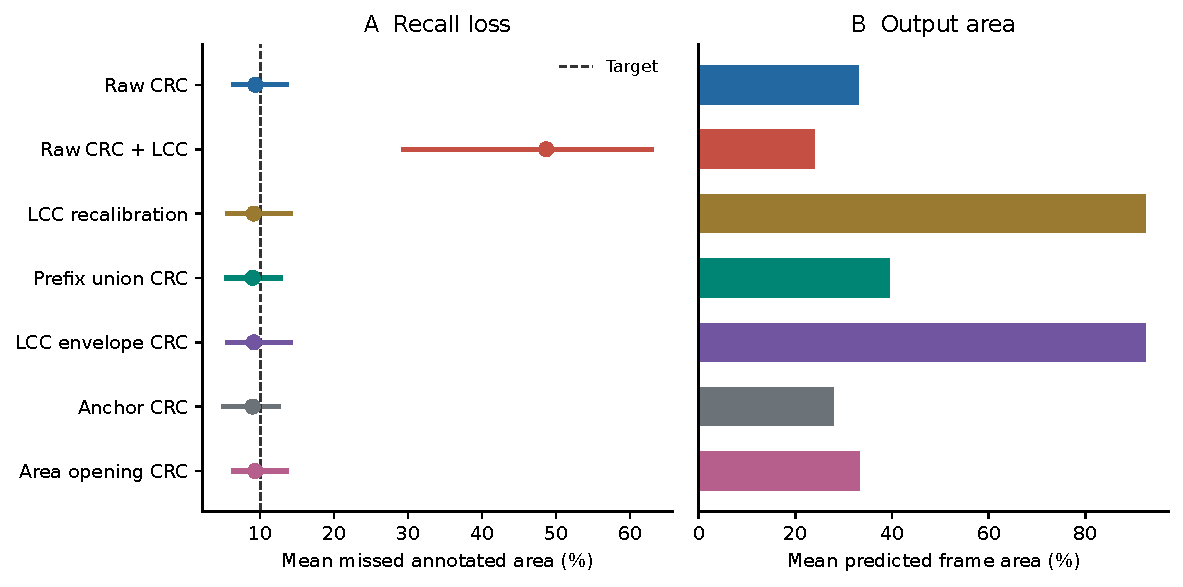
\includegraphics[width=\linewidth]{../figures/primary.pdf}\caption{PraNet evaluation at a 10\% target. Points are split-mean risks; horizontal lines show the central 95\% of risks across overlapping random splits. Bars report mean predicted frame area. The dashed line marks the target.}\label{fig:primary}\end{figure}

\subsection{Recalibration and output constraints}
Persistence CRC attained mean missed area 8.99\% with 39.43\% frame area. The established loss-envelope method attained 9.16\% with 92.54\% frame area while returning an LCC mask. Naive LCC recalibration attained 9.16\%; its empirical performance does not supply a general guarantee for nonmonotone paths. The anchor and area-opening controls attained 9.01\% and 9.35\%, respectively. Figure~\ref{fig:examples} shows two deliberately selected high-penalty cases, chosen by the largest cleanup penalty in distinct source datasets after excluding Kvasir images to avoid acquisition text in the display, rather than representative random images.

\begin{figure}[htbp]\centering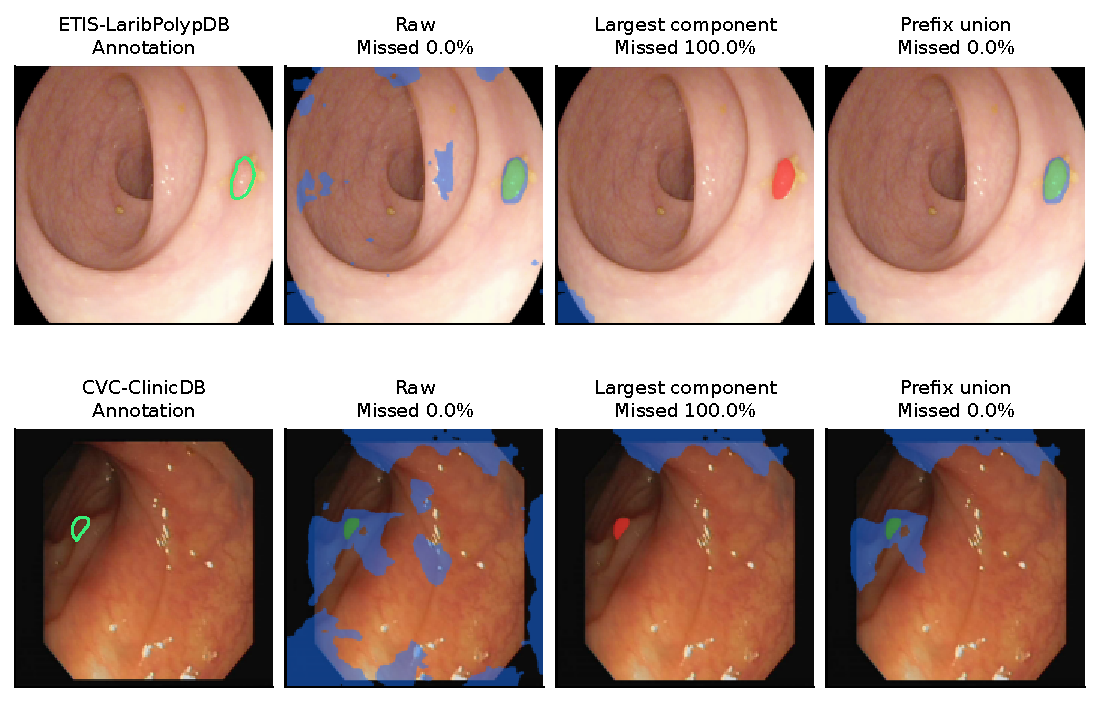
\includegraphics[width=\linewidth]{../figures/examples.pdf}\caption{Two high-penalty PraNet examples at the same descriptive full-pool threshold. Green denotes included annotated area, red missed annotated area, and blue selected background. The prefix union is evaluated at this same threshold for mechanism illustration; its independently calibrated operating point differs. These examples are selected by outcome and do not estimate effect frequency.}\label{fig:examples}\end{figure}

\subsection{Transformer replication and sensitivity analyses}
On Polyp-PVT, the same intervention changed mean missed area from 9.75\% to 13.53\%. Persistence, envelope, and anchor calibration attained 9.78\%, 8.97\%, and 9.82\%, respectively. The transformer had 469/701 nonnested LCC paths and 449/701 paths with an annotated-loss increase. The model comparison changes the magnitude of the effect; neither model is selected on these results.

\begin{table}[htbp]\centering\small
\caption{Polyp-PVT replication at the 10\% target, with the same images and 500 paired splits. All numerical columns except Dice are percentages; split ranges are partition sensitivity.}
\label{tab:pvt}\begin{tabular}{lrrrr}\toprule
Procedure & Missed area & Split range & Frame area & Dice\\\midrule
Raw CRC & 9.75 & 7.31--12.67 & 8.91 & 0.822 \\
Raw CRC + LCC & 13.53 & 10.89--16.33 & 8.59 & 0.818 \\
LCC recalibration & 10.11 & 7.44--13.55 & 18.33 & 0.729 \\
Prefix union CRC & 9.78 & 6.76--12.90 & 10.06 & 0.807 \\
LCC envelope CRC & 8.97 & 4.97--12.44 & 98.48 & 0.131 \\
Anchor CRC & 9.82 & 6.89--13.55 & 11.51 & 0.785 \\
Area opening CRC & 9.75 & 7.27--12.69 & 8.90 & 0.822 \\
\bottomrule\end{tabular}\end{table}

At the primary target, naive LCC recalibration and envelope calibration selected the same grid index in 500/500 PraNet splits. At the primary target, naive LCC recalibration and envelope calibration selected the same grid index in 32/500 Polyp-PVT splits. Naive recalibration had mean Polyp-PVT risk 10.11\%, slightly above the 10\% target; the split variability and finite Monte Carlo experiment do not establish a systematic target violation. Consequently, the experiment demonstrates failure of transferring raw-mask calibration through cleanup, but does not establish that naive final-mask recalibration fails empirically at this target.

For PraNet with four-connectivity, raw/cleaned mean missed areas were 9.36\%/48.64\%; persistence/envelope/anchor risks were 8.99\%/9.18\%/9.01\%. For PraNet with 513-point grid, raw/cleaned mean missed areas were 9.64\%/45.93\%; persistence/envelope/anchor risks were 9.49\%/9.50\%/9.47\%. The target sensitivity results and source-held-out stress results are included in Appendix~\ref{app:additional}.

The classical anchor control used less mean frame area than persistence in the primary PraNet comparison (28.01\% versus 39.43\%) and attained a higher mean Dice (0.579 versus 0.300). Thus the running-union construction is useful for preserving a display-history constraint, but the data do not support preferring it over established increasing filters solely for segmentation utility.

